\chapter{Introduction}
\section{An Overview of Phase-Shift Profilometry}
\subsection{General Description}

Three-dimensional (3D) imaging techniques have a wide array of applications in medicine, manufacturing, entertainment, etc \cite{Guo2009}. 
Its most common application is in the digital archiving of cultural heritage sites and objects due to its non-invasive and non-contact approach \cite{Simon2013}. 

Several methods for digital 3D reconstruction have been developed for the past years. Among these methods, the structured light illumination technique, particularly phase-shift profilometry (PSP), has proven to be a simpler and cheaper yet promising method for 3D reconstruction of surfaces as compared to laser scanners and other expensive tools used in 3D imaging \cite{Zhang2006, Moreno}. 

PSP is a fast-acquisition 3D shape measurement technique which provides high-resolution (pixel-rich) images appropriate for the study of small details in an object \cite{Stoykova2008}. 
A PSP system consists of a projector used for projecting phase-shifted sinusoidal fringes onto the object and a camera for recording the fringe image \cite{Chen2012}.

\subsection{Related Works}

Previous works on camera-projector pairs deal with their calibrations separately \cite{Fernandez}, removal of vignetting effect through per-pixel point correction \cite{Yu2004} or only for fixed camera settings \cite{Goldman2010}, and computing for the nonlinearity or gamma factor itself \cite{Wang2014}, etc. 
These methods prove to be either limited or complex for camera-projector pair calibration depending on the approach.

In the Philippines, as far as we know, PSP has been used twice for applications in the study and archiving of a heritage site and object. 
The first one was in 2010 wherein Vergara used PSP for the archiving of the Angono petroglyphs (see fig. \ref{fig:angonosite}) \cite{Vergara2010}. 
In his thesis, he was able to reduce the artifacts introduced by the PSP system using low intensity fringe patterns to avoid the non-linear regions of the camera-projector pair and by setting the camera aperture to the smallest possible size to reduce vignetting effect. 
He was also able to lessen the singularities by proposing a specified PSP system geometry but was not able to completely remove them. 

\begin{figure}[h!]
	\centering
	\subfigure[Angono petroglyphs]{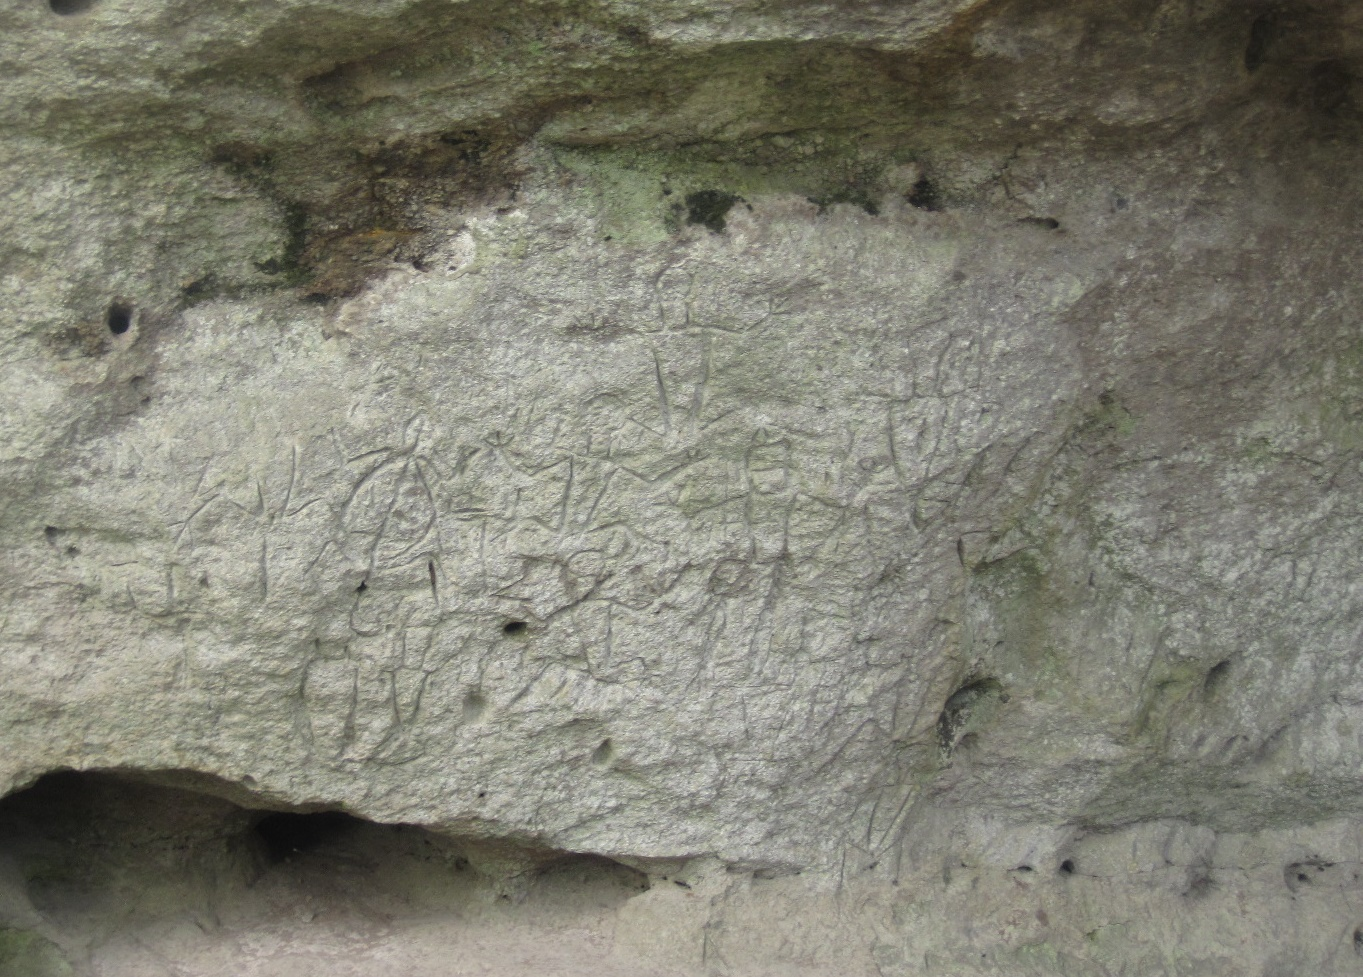
\includegraphics[width=0.45\textwidth]{figures/angono3.jpg}\label{fig:angonosite}}
	\subfigure[Ticao stone]{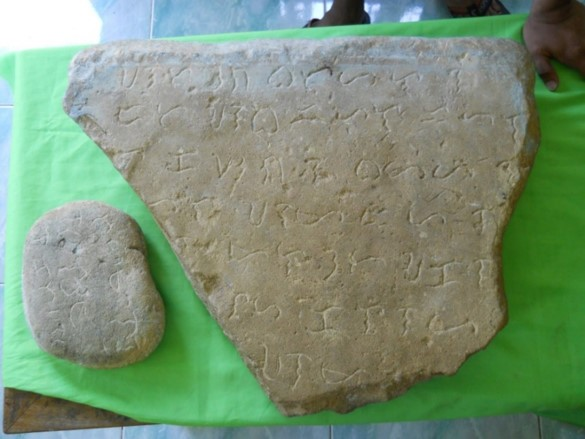
\includegraphics[width=0.45\textwidth]{figures/ticao.jpg}\label{fig:ticao}}
	\caption[Angono petroglyphs and Ticao stone]{(a) Angono petroglyphs in Binangonan, Rizal \cite{Vergara2010} and (b) Ticao stone from Masbate \cite{Sze2012}.}
	\label{fig:angonoticao}
\end{figure}

The second application was in the study of the graving marks of Ticao stone (see fig. \ref{fig:ticao}) in 2012 in which Sze focused on phase-to-height conversion using Du and Wang's algorithm to measure the probability distribution of the graving depths and widths but was not able to address the source of singularities and artifacts \cite{Sze2012}.

The novelty of this research is its easy-to-implement algorithms for the complete removal of artifacts and singularities which utilizes the response curves of the camera-projector pair for non-repetitive calibration as well as a geometry-independent PSP setup which need not have fixed settings.

%as well as a geometry-independent and mobile PSP set-up which we can easily use for in-situ experiments.

\subsection{Statement of the Problem}

Depending on the PSP system, an uncalibrated PSP has several artifacts which are carried out in the 3D reconstruction. 
In digitization of petroglyphs in which rock art details can have shallow depths, the details are obstructed due to these artifacts, and in worst cases, they can no longer be retrieved from the unwrapped phase maps.

The aforementioned artifacts arise from optical and digital nonlinearities of both the projector and camera such as vignetting effect or nonuniform illumination of light and inherent gamma \cite{Liu2010, Gorthi2010, Juang2007}. 
As a consequence, phase value at a particular image point may change resulting to a wrong depth or height perception of
the object upon phase retrieval.

Another source of artifact which need to be addressed are the projected sinusoidal fringes which are left behind in the unwrapped phase and causes reduction of observed details.

Figures \ref{fig:vergara} and \ref{fig:sze} show some of the phase maps and 3D reconstructions of characters in the Angono petroglyphs and Ticao stone from Vergara's \cite{Vergara2010} and Sze's \cite{Sze2012} thesis, respectively. In these figures, we see the artifacts that were not remove in the digital reconstructions such as the vignetting effect and the sinusoidal fringe artifacts.

\captionsetup[figure]{width=5in}
\begin{figure}[h!t]
	\centering
	\subfigure[]{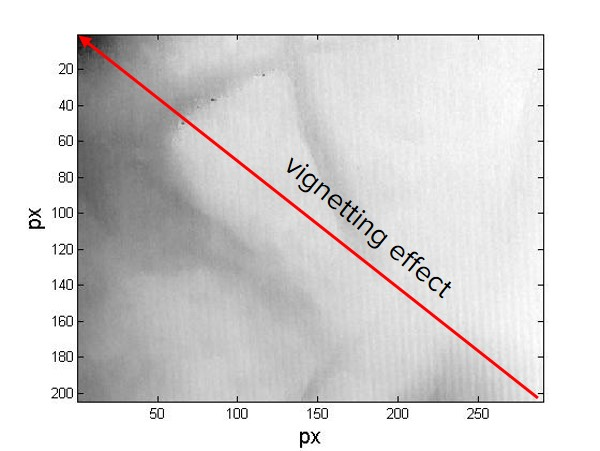
\includegraphics[width=0.425\textwidth]{figures/vergara2D.jpg}\label{fig:verg2D}}
	\subfigure[]{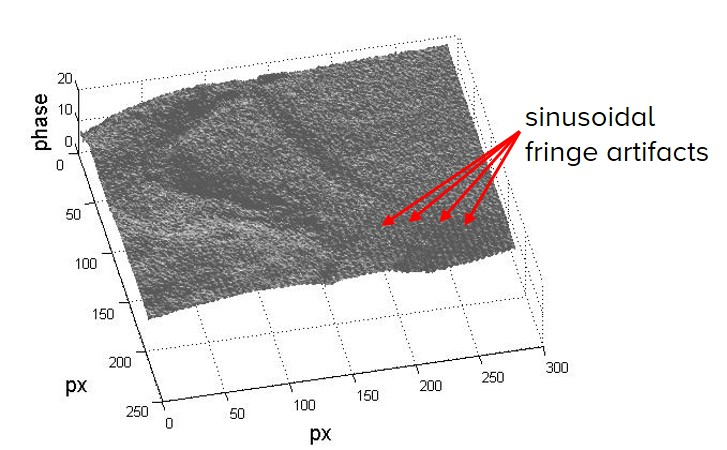
\includegraphics[width=0.55\textwidth]{figures/vergara3D.jpg}\label{fig:verg3D}}
	\caption[Reconstructions from Vergara's thesis]{Reconstructions of a  character in the Angono petroglyphs from Vergara's thesis in 2010 \cite{Vergara2010}. The arrow for the vignetting effect shows the direction of the nonuniform illumination of light. Fringe artifacts are also visible in the 3D reconstruction.}
	\label{fig:vergara}
\end{figure}

\captionsetup[figure]{width=5in}
\begin{figure}[h!t]
	\centering
	\subfigure[]{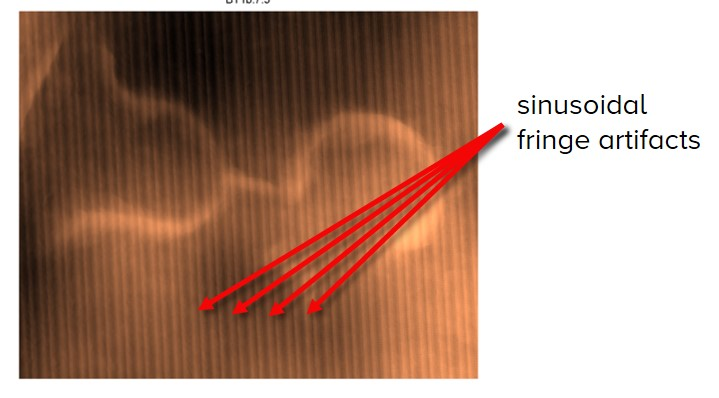
\includegraphics[height=0.3\textwidth]{figures/sze2D.jpg}\label{fig:sze2D}}
	\subfigure[]{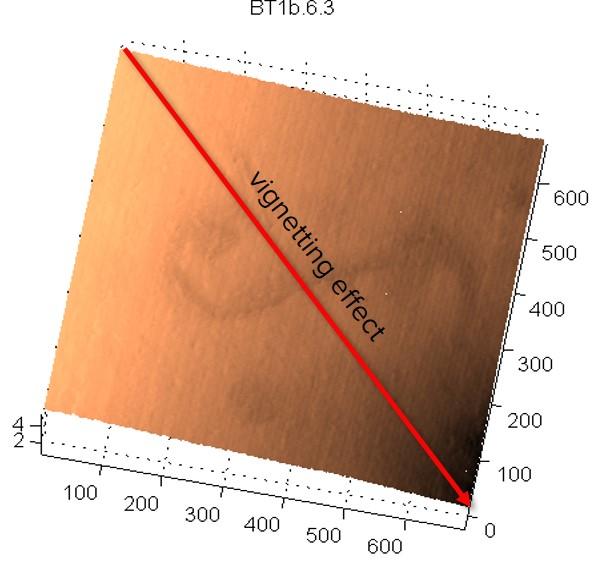
\includegraphics[height=0.35\textwidth]{figures/sze3D.jpg}\label{fig:sze3D}}
	\caption[Reconstructions from Sze's thesis]{Reconstructions of some of the characters in the Ticao stone from Sze's thesis in 2012 \cite{Sze2012}. The sinusoidal fringe artifacts are very visible in the phase map. Vignetting effect obscures the details in the digital 3D object.}
	\label{fig:sze}
\end{figure}

Lastly, phase unwrapping method for PSP is a crucial step as it gives the absolute phase for direct conversion to actual height (depth). For typical unwrapping of phase along one dimension, discontinuities may occur causing singularities\footnote{Singularities are points in 2D and lines in 3D which introduce sudden jumps in the phase map after phase unwrapping} to form in the phase maps \cite{Ortega2009}.
Efficient phase unwrapping which operates in 2D must then be used so as not to generate these discontinuties. Quality-guided path unwrapping algorithm following a noncontinuous path by Herraez et al. was used for phase unwrapping instead of the typical unwrapping in 1D \cite{Herraez2002}.

These artifacts combined greatly affect the quality of 3D reconstruction using PSP as seen in the reconstructions.
Hence, step-by-step calibration for removing these artifacts needs to be implemented in order to get the most detailed 3D reconstructions. 

\section{Motivation of the Study}

The Angono petroglyphs dated to be not later than 1500 B.C. (late Neolithic era) is one of the country's oldest natural heritage sites \cite{Unesco2006}. There have been several attempts of archiving all the 127 characters in it through different methods. Jesus Peralta was the first to document the petroglyphs stencils of the characters and traced them manually \cite{Peralta1973}. 

Vergara was only able to archive a few of the characters in the Angono petroglyps. In a most recent work, laser scanning of the site was done by a company outsourced by the National Museum but the details are not pixel-rich and the characters are not observable.

This study is geared towards the archiving of all the Angono petroglyph characters including the latest graffiti in a pixel-rich and artifact-free digital 3D reconstruction such that we can study the individual characters thoroughly without the need to touch them. 

The digital 3D data will be made available to the public through open source 3D viewing software such that anyone can readily view it. Also, the heritage centers (e.g. National Museum) protecting the site may use it for future restoration and the like.

A mobile and stable PSP setup which we can easily use for \textit{in-situ} experiments was also created to reduce assembly time. The setup includes a portable platform which can contain both the projector and camera.

\section{Thesis Structure}

This thesis contains 7 chapters including the Introduction. Chapter 2 discusses the PSP technique, the schematic setup of a PSP system, and  general algorithms used to extract the phase and actual height of a target object. 

Chapter 3 introduces the inherent gamma of projectors and camera, how it affects the quality of the 3D reconstruction, and the processes done to correct it though curve fitting and interpolation. 
Chapter 4 proposes different background subtraction techniques for the removal of all vignetting effects in the unwrapped phase maps. 

Chapter 5 discusses the concept of Fast Fourier Transform (FFT) filtering and how it is applied to the resulting phase maps to remove the sinudoidal fringe artifacts.
Chapter 6 shows the results of the calibrated PSP method on 1:1 scale model of some characters in the Angono petroglyphs engraved in styrofoam boards and the 3D reconstruction of the test object with phase-to-height conversion. 

The summary of this thesis and recommendations for future work are presented in Chapter 7.

%The purpose of this thesis is two-fold: (1) to deliver an analysis of parallel computing specifically on a self-constructed computer cluster; and, (2) to provide an instruction manual for other researchers so that they can set up their own affordable HPC clusters.